\documentclass[a4paper]{article}

\usepackage{fullpage}
\usepackage{graphics}
\usepackage{multirow}
\usepackage[table]{xcolor}
\usepackage{graphicx}
\usepackage{pdfpages}

\newcommand{\fixedland}{{\it Fixed Landmarks}}
\newcommand{\challenge}{\paragraph{Challenge}}
\newcommand{\method}{\paragraph{Method}}
\newcommand{\approach}{\paragraph{Proposed Approach}}
\newcommand{\citep}{\cite}

\title{Image Analysis and Modelling of the Vascular Tree:\\Application to the Automatic Quantification of\\Vascular Stenoses and Aneurysms and the\\Choice of Patient-specific Stents}
\author{Concours CNRS 2012 -- Section 7\\Projet de Recherche}
\date{R\^omulo (TEIXEIRA DE ABREU) PINHO}

\begin{document}

\maketitle

\begin{noindent}
{\em Obs: I am a Brazilian native who has been living in France for two years. Despite my working knowledge of the French language, I am writing this project proposal in English, for efficiency reasons.}
\end{noindent}

\begin{abstract}
\hrule
\medskip
Atherosclerosis figures as one of the leading cardiovascular diseases, which remain as the major cause of death in developed countries. Image analysis and processing is an important tool in the diagnosis and treatment of vascular diseases. Minimally invasive interventions are increasingly becoming the treatment option of choice, given the reduced surgical risk for the patient. A good example is the use of stents to reopen vascular stenosis or to protect the dilated walls of aneurysms from further expansion. Stent choice remains, nevertheless, a subjective decision. An inadequate stent may migrate to another location, may exert exaggerated pressure on the vessel walls, may not properly cover the affected area, etc. This document describes a project proposal for the automatic detection and quantification of stenosis and aneurysms and for the automatic prediction of optimal patient-specific stent parameters. The proposed methods build upon the work presented in my PhD thesis, which focussed on the assessment and stenting of tracheal stenosis. They also integrate physical properties of blood vessels and stents, as well as stent deployment and blood flow simulations, into the stent choice process. 
\medskip
\hrule
\end{abstract}


\tableofcontents

\pagebreak

\hrule
\section{Context}
\hrule

\medskip
\medskip

Atherosclerosis is a pathology of the blood vessels that occurs when substances such as fat and cholesterol accumulate in the vessel walls, forming plaques. These plaques cause stenoses (vessel narrowing) and aneurysms (weakening and swelling of the vessel wall). Such conditions may lead to severe consequences, for example heart attacks, strokes, and the rupture of the vessel wall, all of them life threatening \citep{Gennest,Libby}. Atherosclerosis figures as one of the leading cardiovascular diseases, which remain as the major cause of death worldwide \citep{WHO}. 

Concomitantly, the use of images plays a very important role in the diagnosis, treatment, and follow up of vascular diseases. Likewise, minimally invasive interventions are becoming more available and are the preferred treatment option given the reduced surgical risk to the patient. The treatment of atherosclerosis using stents is a very good example that profits from both the use of images and minimally invasive interventions. 

A large variety of stents is available in the market. However, choosing the correct stent parameters (type, length, diameter, and deployment location) is challenging and remains a specialist-dependent and subjective task, which is mostly based on the expertise of the physician in charge. This problem attracts large attention. The multi-centre, EU-project THROMBUS\footnote{http://www.thrombus-vph.eu/}, for instance, is an attempt to understand the formation of thrombosis in cerebral aneurysms after stent implants, in order to improve stent design, choice, and deployment. An event to compare the results of existing algorithms to aid in the detection and quantification of coronary stenoses will also soon be organized\footnote{http://coronary.bigr.nl/stenoses}.

In my PhD thesis, I showed that the choice of stents for the treatment of tracheal stenosis can be automated and simplified with the use of active shape models (ASM) \citep{Cootes}. The proposed method solves the problem of automatically determining the location of the stricture, its length, and the degree of narrowing by giving an estimation of the patient's healthy trachea, that is, if stenosis were not present. From this estimation, followed by a segmentation of the narrowed trachea, determining the parameters of the stenosis and consequently of the {\em patient-specific} stent becomes a straightforward task. 

Many challenges exist when trying to use the ASMs of healthy shapes in the cardiovascular domain. First and foremost, to build the model, it is necessary to segment a large collection of healthy vascular trees and establish point-wise correspondences between them. The {\em automatic segmentation and labelling of the vascular tree} remains an open problem \citep{ORKI-08,Antiga,CARR-07,Scherl200721,Bemmel,Dikkers}. Furthermore, the {\em statistical analysis of tree-like shapes} is still in its early stages \citep{Feragen}. 

Another challenge is that when optimizing the stent choice, several parameters need to be taken into account, such as the physical properties of the vessel wall and of the stents themselves and the estimation of the blood flow after deploying the stent. In cerebral aneurysms, other constraints with respect to scale and stent properties are further taken into account \citep{larrabide:2439,Larrabide2010,bogunovic:210,zhang:1294}, although the philophy is the same as in, e.g., coronary stents. To the best of my knowledge, such parameters have only been studied in post-stent-deployment scenarios or in simulations \citep{deBeule,Florez2,Gori,Vuk,FLOR-07b,Sforza}, but have never been integrated in an {\em automatic stent choice process}, especially one that is based on ASMs. 

This project therefore aims at studying and solving the problems above and at evaluating the solutions through simulations and in the clinical domain. In order to achieve it, I would like to be part of the {\em Centre de Recherche en Acquisition et Traitement de l'Image pour la Sant\'e} (CREATIS), whose expertise in the domain of segmentation of images of the vascular system and in the use of stents in the treatment of vascular stenoses and aneurysms will be an invaluable contribution.

\medskip
\medskip

\pagebreak

\hrule
\section{Project Description}
\hrule

\medskip
\medskip

The objective of the proposed project is to develop a solution for the problem of automatic quantification of stenosis and stent choice in the treatment of vascular stenoses and aneurysms. To date, such problem has only been solved with semi-automatic methods \citep{Gremse01092011,Scherl200721,HERN-06b,Bemmel}. The goal is then to improve previous solutions with an {\em automatic} process that optimizes the {\em patient-specific} choice of stent type, length and diameter. The following sections present the main challenges involved in the project and the approaches to solve them. 

\subsection{Estimation of Healthy Vessels}

\challenge
When assessing vascular stenoses or aneurysms, physicians tend to pick healthy regions around the affected area in order to quantify the parameters of the deformation (extension, severity). These healthy regions in fact act as an estimation of the vessel if it were completely healthy. However, the simple selection of healthy sections may overlook shape characteristics, such as curvature, and vessels' physical properties, such as elasticity, malleability, and bending. The choice of the healthy vessel section is in fact a way to estimate the shape of the pathological region if the pathology were not present. In other words, physicians intuitively estimate how the vessel would appear if it were healthy. By doing this, they have a clearer image of the parameters of the deformation, which aids them in determining the stent dimensions and deployment location.

The {\em estimation of this healthy shape} is very subjective, much dependent on the expertise of the physician in charge. It would be desirable to devise a method in which such estimation is done automatically, taking into account the physical and geometrical properties of vessels and stents.

\approach
In \citep{Pinho:Trachea4}, a method for the estimation of healthy tracheae from CT images of patients suffering from tracheal stenosis was proposed. This method is based on the construction of an active shape model (ASM) \citep{Cootes} of 3D surfaces of healthy tracheae allied with a new model fitting algorithm, called \fixedland. When the model is registered to a CT image volume of a patient with tracheal stenosis, it is capable of matching the parts of the tracheal wall that are healthy while at the same time estimating the shape of the remaining parts as if they were healthy. The \fixedland\ algorithm is responsible for avoiding the narrowed parts of the patient's trachea, enabling the statistical model to generate a plausible healthy tracheal shape.

A natural extension of the work above is the application of the proposed 3D ASM in the cardiovascular domain. Since vessels, as well as tracheae, are objects of tubular topology, and the shape characteristics of their stenoses are roughly the same, it is intuitive to believe that the method will also be able to estimate the shape of healthy vessels from images of patients with vascular stenosis. This rule also tends to apply in the case of aneurysms, as long as there are enough healthy regions around the location of the swelling.

In this project, the method proposed for the trachea will be adapted and extended so that it can be used with narrowed and swelled vessels. In the first instance, a training set of healthy vessel sections will be built using segmentation methods available in the literature, for example \citep{Florez2}. In this way, the problem is reduced to modelling objects of tubular shape, without bifurcations, resembling the case of the trachea. Since healthy vessel sections tend to appear with good contrast in the images, their segmentation is in principle a relatively straightforward task. 

The main difficulty lies in the segmentation of the vascular tree and the corresponding surface representation to be used in the statistical model. To the best of my knowledge, very little has been done in the field of {\em statistical shape models of tree-like structures} \citep{Feragen}. In the next phase of the project, existing surface representation methods \citep{Florez, Antiga} and the corresponding branch nomenclature will be employed so as to establish correspondences between the shapes of the statistical model's training set, which is an important step in the model construction. Existing ASM fitting algorithms will be extended to cope with the possible new difficulties when registering the model to deformed vessels. New fitting algorithms will also be developed to account for bifurcations. At this stage, only geometrical properties of the vessels will be taken into account. The inclusion of physical properties of vessels and stents in the model are discussed later in the text. 

\subsection{Segmentation of the Vascular Tree}

The segmentation of the vascular tree has been a topic of study for quite some time, but the automatic segmentation remains an open problem \citep{ORKI-08}. In the context of this project, the segmentation task is subdivided into two objectives: 1) the segmentation of healthy vascular trees; 2) segmentation of vessels with stenosis. Each is detailed in the following sections.

\subsubsection{Healthy Vascular Trees}

\challenge

ASMs depend on the selection of a large set of training shapes, whose geometrical variation is encoded in the model. The segmentation of the healthy vascular tree is thus an important step in the construction of the model. 

\approach

This segmentation problem has much in common with the segmentation of the airway tree. Despite also being an open problem, automatic segmentation algorithms for the airways exist and were even been evaluated in a recent segmentation challenge\footnote{http://image.diku.dk/exact/}. One of these algorithms \citep{Pinho:Airways2} implements an iterative region growing with adaptive, cylindrical ROIs that employs anatomical information in the detection and elimination of leaks, a common problem in region growing. The method also includes an initialization step to automatically detect the starting point of the trachea, which is given as a seed point to the region growing algorithm. 

%\begin{figure}%
%\centering
%\includegraphics[width=0.5\columnwidth]{research_interests_airways.jpg}%
%\caption{Segmentation of the airway tree as proposed in \citep{Pinho:Airways2}.}%
%\label{fig:airways}%
%\end{figure}

The intention is to adapt and extend the referred method to the segmentation of healthy vessels and to compare it with other (semi-)automatic methods \citep{Zhou20121,CARR-07,FLOR-07b,Florez2,Scherl200721,Antiga,Bemmel}. In order to detect a seed point for the region growing algorithm, tube enhancement filters \citep{ORLO-09} may help in at least isolating the tubular structures in the image, from where the detection process may be triggered. 

\subsubsection{Pathological Vessels}
\label{sec:narrowedarteries}

\challenge
Similarly to the case of tracheal stenoses, segmenting the narrowed vessels is an important step in the automatic calculation of the parameters of the vessel stricture. Previous experience with the segmentation of the trachea, however, has demonstrated that the segmentation of narrowed tube-like structures in medical images may be difficult \citep{Triglia,Pinho:Trachea7}. Region growing, for example, tends to fail to recover the correct tube wall if the narrowing is too severe and the lumen is not completely visible in the image. 

\approach

In \citep{Pinho:Trachea4}, an estimation of the patient's healthy trachea was used as initialization of a deformable model to segment the narrowed tube. The proposed deformable model, based on the snake model proposed by \citep{Kass}, was able to correctly segment the tracheal wall even in the more difficult cases. 

I will thus experiment with the referred deformable model in order to automatically segment narrowed vessels. The idea will still be to initialize the model with the estimation of the healthy vessel obtained with the ASM. This method should give better results then other solutions in the literature \citep{CARR-07,Florez2,Antiga,Bemmel}, but an in-depth comparison with those algorithms will be necessary.

\subsection{Stent Choice}

Physicians intuitively estimate the healthy shape of the narrowed vessel when quantifying the stenosis or the aneurysm. The solutions proposed above should be able to mimic the physician's work in a methodological and mathematical manner. After the estimation of the healthy vessel shape, we are ready to automatically detect the exact location of the stenosis and to quantify it. For this, it is necessary to track changes in the cross-sectional area of the narrowed tube relative to the estimated healthy tube \citep{Pinho:Trachea4} or relative to selected healthy vessel sections \citep{Florez2,Bemmel}.

Once the stenosis or aneurysm has been detected and quantified, the parameters of the stent are trivially obtained. At this point, the whole chain of the proposed project will be finished. However, the effectiveness of the predicted stent can only be verified after it has been deployed in the patient's vessel. If the stent is inadequate, it may migrate to another location or strain the vessel wall. 

For this reason, I will add to the stent choice process several parameters derived from the physical properties of the vessel and of the stent itself. In addition, every predicted stent will be used in a blood flow simulation step such that its effectiveness can be further verified. From the simulations, other parameters will be extracted and added to the decision process. In this way, the proposed method will be turned into an optimization process on several variables. Some of them will impact the estimation of the vessel's healthy shape, some will impact the stent choice.

\subsubsection{Extending the Statistical Shape Model}

\challenge
The registration of the ASM of healthy vessels to an image of a patient with atherosclerosis is an iterative, edge-based search. At each iteration, the new locations of the landmarks that describe the surface of the vessel are determined and a least squares minimization process makes the shape generated by the ASM fit to the new point locations. Since the model is constrained by the (healthy) shape information contained in it, the resulting surface will resemble a healthy vessel.

A ``healthy vessel'' in this context means that only the geometrical variation about the vessels is captured by the statistical model. Still, vessels have physical properties such as elasticity, malleability, and bending, that are not explicitly encoded in the model. At the best, the geometric information may implicitly contain some aspects of the referred properties. 

\approach
I will then collect the physical properties of vessels available in the literature \citep{ZAHN-11d,BOUS-09c,BOUS-08c,SULA-08a,Oubel,zhang:1294,Balocco} in order to add such information to the 3D ASM. As a result, when registering the model to the patient's image these properties will further constrain the deformation, which should help in obtaining a better estimation of the healthy vessel shape. 

In the same way, I will further extend the ASM with the physical properties of the stents. Since the ultimate objective of the project is the automatic prediction of patient-specific stent parameters, it is reasonable that their physical properties be an extra parameter in the construction of the model. Consequently, when registering the model to the patient's image, not only will the properties of the vessel play a role, but we will at the same time influence the estimation of the healthy vessel with the properties of the stent. The novelty here will be the combination of geometric (shape) and non-geometric information into a multi-dimensional ASM. 

\subsubsection{Physically-based Segmentation of Pathological vessels}

\challenge
In the same way that the statistical shape model can be extended, so can be the segmentation of narrowed and swelled vessels. Originally, the snake model proposed in \citep{Kass} depends on internal and external energies to deform the surface towards the desired image feature. The internal energies take only elasticity and bending into account. 

\approach
I will add extra energy terms taking into account vessels' physical properties \citep{BOUS-09c,ZAHN-11d}, in order to restrict (or improve) the surface deformations, so that the model can better adapt to the vessels' boundaries. Such physical properties must also take into account those of narrowed and swelled regions, since the main object of this segmentation step is to correctly segment them.

\subsubsection{Simulations}

\challenge
As stated previously, when the estimated healthy vessel shape and the segmented narrowed vessel are obtained, the automatic detection and quantification of the stenosis or aneurysm tends to be trivial. The stent to be chosen, however, is the one that will optimize the blood flow after deployment. 

Blood flow simulations already play an important role in stent design and placement planning \citep{deBeule,ATTI-08}. They are also extensively used for flow assessment after stent deployment \citep{Vuk,Gori}. However, to the best of my knowledge, such simulations have not yet been integrated in a method or algorithm for the stent choice process. 

\approach
In \citep{Florez,deBeule}, methods were proposed for stent deployment simulations using deformable models and numerical methods. With these methods, it is possible to (visually) verify whether the predicted stent properly expands the narrowed region of the vessel or whether it correctly bypasses the swelled region. 

The idea is then to methodologically quantify these parameters, by using the stents' and vessels' physical properties, and to have measures for, e.g., vessel wall straining, stenosis/aneurysm coverage, stent deformation, etc \citep{BOUS-09c,BOUS-08c,SULA-08a}. These parameters can be further added to the ASM so as to improve the healthy shape estimation. Consequently, the ASM registration will tend to yield a shape with the best characteristics in terms of the stent vs. wall interaction as well.

To achieve the integration of blood flow simulation with the stent choice, the plan is to define a function of the blood flow subject to the stent parameters (physical properties, deployment location, length, and diameter). This function will then be maximized, such that the chosen stent is the optimal one for a certain patient. This optimization process will thus influence the entire workflow, from the estimation of the healthy vessel shape, passing through the segmentation of the narrowed/swelled vessel, to the detection and quantification of the stenosis/aneurysm, and the final prediction of the stent parameters. In fact, we imagine an algorithm that implements the workflow depicted in Figure \ref{fig:workflow}. 

\begin{figure}%
\centering
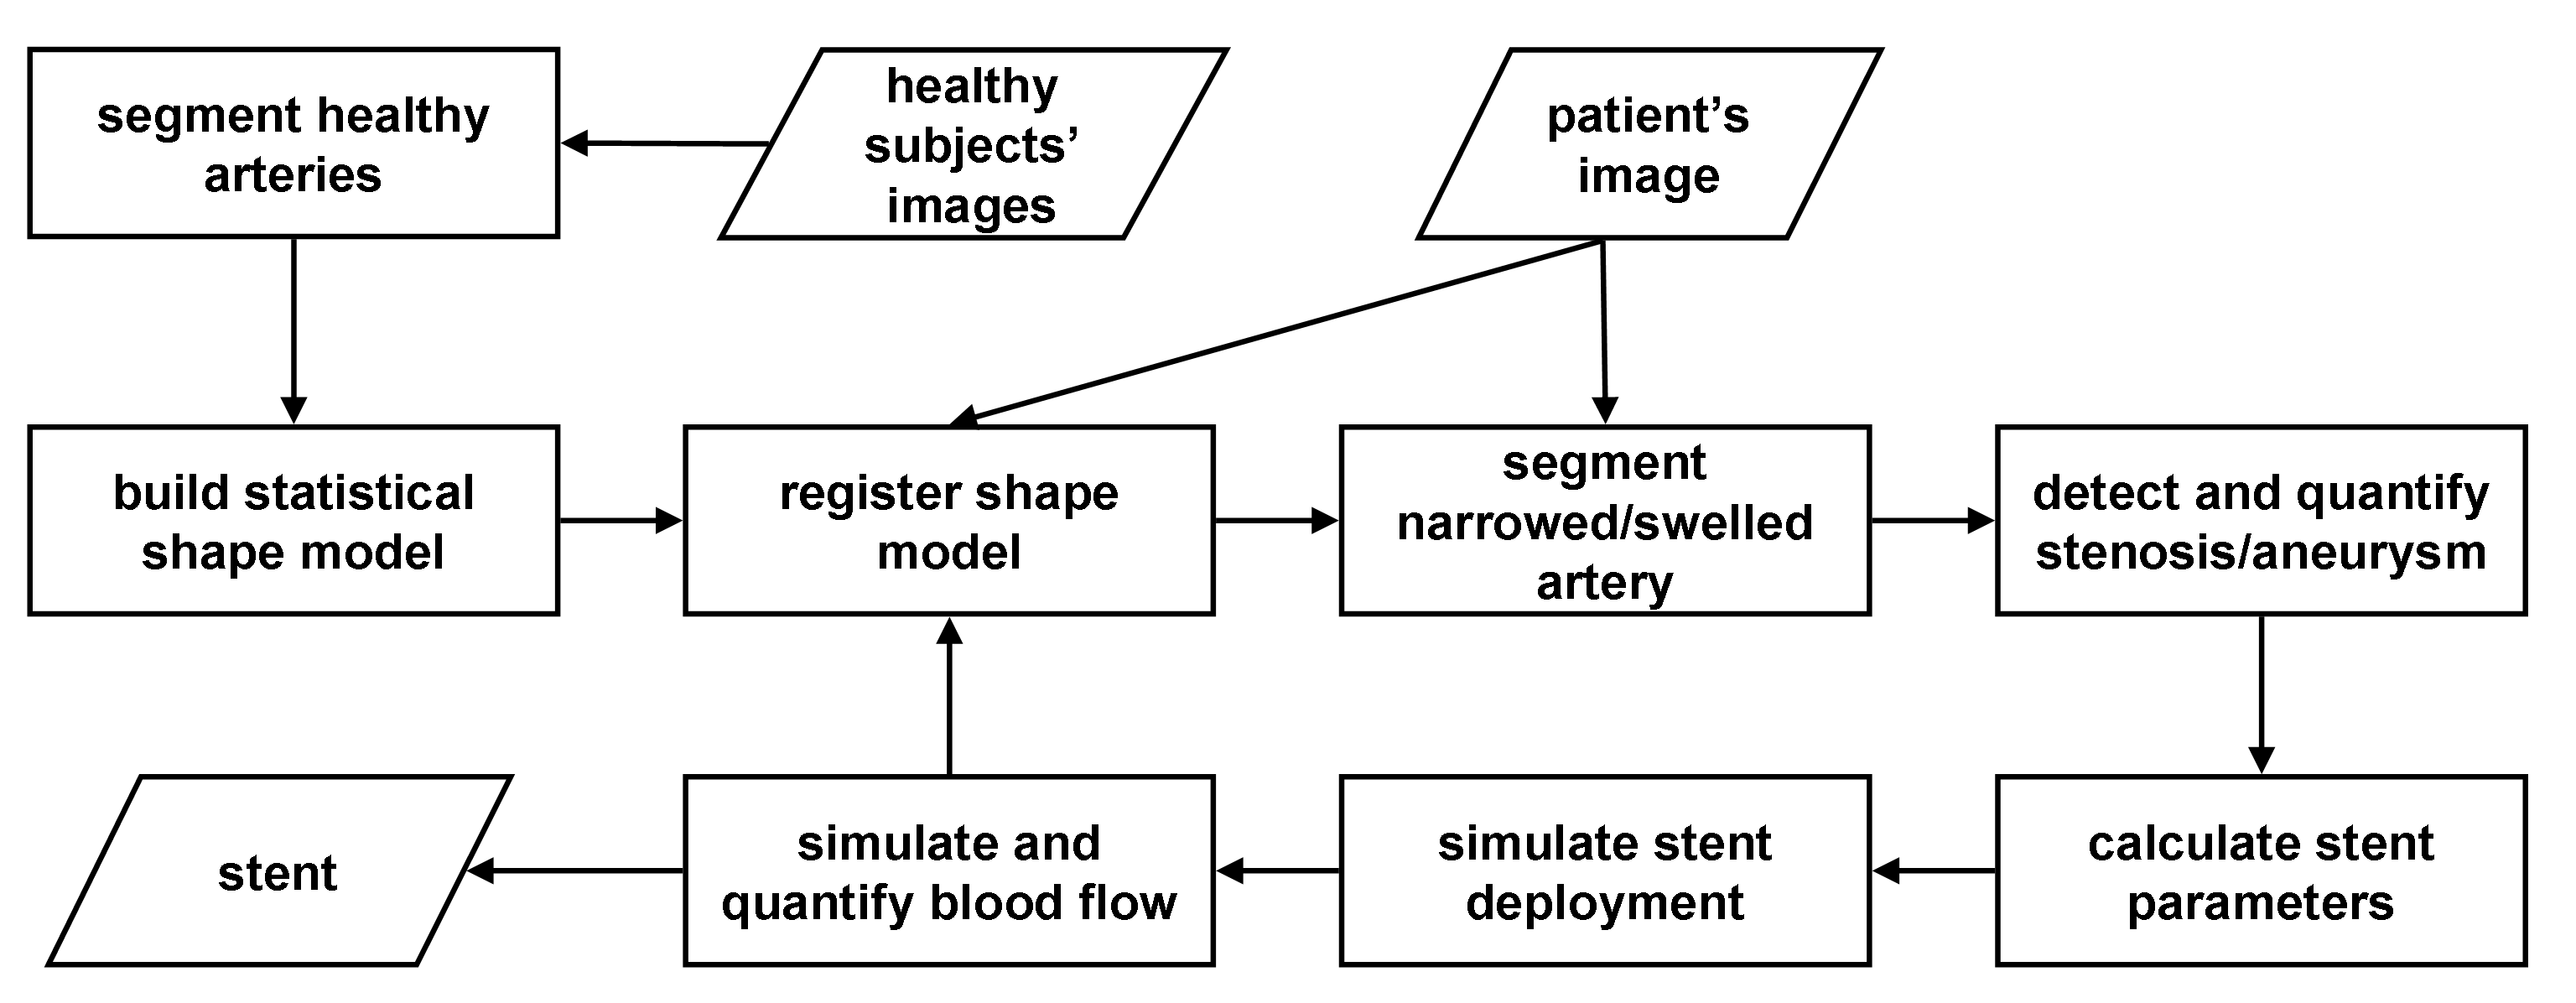
\includegraphics[width=0.8\columnwidth]{workflow.png}%
\caption{Workflow of the complete automatic stent prediction process.}%
\label{fig:workflow}%
\end{figure}

\subsection{GPU Acceleration}

\challenge
In order to achieve the expected results with the proposed methods, a lot of computational power may be necessary. The blood simulations, for instance, are very computation intensive (e.g., 48 hours running on a 200-CPU cluster \citep{deBeule}). The proposed optimization process, as well, is a classic case study for the use of clusters and grids, given the number of potential variables in the problem. I envision the use of such architectures, but bringing them to the clinic is impractical and expensive. A more viable, yet powerful, solution is thus necessary.

The FASTRA\footnote{http://fastra.ua.ac.be/en/index.html} technology is a successful attempt of building a desktop supercomputer using multiple GPUs. At the cost of a couple of high-end desktop computers, this technology yields computing power comparable to more than 256 CPUs working together, with proper GPU programming.

In GPU programming, however, the size of the data to process may be larger than the available GPU memory. In this case, we need to be selective about which parts of the data should be transferred to the GPU memory at each time. In this project, it is possible that the areas of interest in the image, that is, those with the vessels under study, occupy a small part of the image. Careful identification of this part of the image could minimize data transfers between RAM and GPU. 

\approach
In \citep{Pinho:Cache1}, a similar problem was dealt with, but in a different scale. Since image processing pipelines may require several simultaneous copies of the image buffer, current available RAMs may not be large enough. An out-of-core solution for image processing based on sliding window cache and pre-fetching techniques was then proposed. In other words, only the parts of the image that are necessary in a given moment reside in main memory. The other parts remain in disk. Using a-priori knowledge about the image traversal pattern of image processing algorithms, it is possible to predict which regions of the image will be needed in the future. These images can be asynchronously fetched from disk and stored in a cache before being requested by the algorithm. If the I/O operation is fast enough, it is very likely that the algorithm will not have to wait for the request complete. 

The method above can similarly be applied in the selection of what data to bring to the GPU. I will then analyse the image traversal patterns of the algorithms developed in this project and develop new cache and pre-fetching strategies for the GPU vs. RAM architecture. In this way, the stent choice optimization can potentially be made in the clinic without the need of the cluster structure.

\medskip
\medskip
% \pagebreak
\hrule
\section{Integration in the Laboratory, Collaborations, Schedule}
\hrule

\medskip
\medskip

\subsection{Laboratory}

My intention of joining the CREATIS group is on the one hand to benefit from their expertise in the several areas correlated to this project proposal. In particular, CREATIS is the lead group of the multi-centre, EU-project THROMBUS, which focusses on the improvement of stent choices in the treatment of cerebral aneurysms. In addition, the group has large experience in the domain of segmentation of the cardiovascular system \citep{BARB-11c,Florez2,FLOR-07b,ORKI-08}, assessment of stenosis \citep{HERN-06b} and simulations and measurements related to stent deployment \citep{Florez,ATTI-08,ZAHN-11d,BOUS-09c,SULA-08a}. On the other hand, it will be my role to contribute to group's expertise by bringing to the lab my own experience with the automatic assessment and patient-specific stenting of tracheal stenosis and applying it to the cardiovascular domain.

CREATIS also have at their disposal an internal computer cluster and the computation power of the {\it Centre de Calcul de L'Institut National de Physique Nucl\'eaire et de Physique des Particules} (CC-IN2P3). Their expertise in the parallel computing domain and the processing of massive image data with GPUs have been demonstrated through their participation in projects such as the Virtual Imaging Platform (VIP)\footnote{http://www.creatis.insa-lyon.fr/vip} and hGate\footnote{http://hgate.opengatecollaboration.org/}. Such expertise and tools will be invaluable for the simulation parts of the proposed project. 

Most importantly, CREATIS also profit from a very multidisciplinary nature and strong links with the clinical practice, most notably that of the {\it h\^opital neuro-cardiologique des Hospices Civiles de Lyon} (HCL) and of the {\it Centre L\'eon B\'erard} (CLB). This will give me the opportunity to evaluate the results of the proposed project with real patient data and to have immediate feedback from physicians. 

\subsection{Collaborations}

During my PhD in Belgium, I established a very good relationship with Prof. Dr. Jan Sijbers, my thesis supervisor, in the VisionLab group of the University of Antwerp. The group has extensive experience with medical image segmentation problems and modelling of cylindrical objects, which could be interesting in the context of this project. In addition, this is the group where the FASTRA technology for GPU acceleration was developed, and they are always interested in new applications for it. I would like to bring the VisionLab and CREATIS together during the course of the proposed project, so that they can benefit from each other's work.

My stay in Belgium also allowed me to get acquainted with the work of the Stent Research Unit of the University of Ghent. Since their work is focussed on the design of stents using numerical simulations, on which much of this project may be based, it is a potential collaboration opportunity. 

I also envision collaborations with the academic and industrial partners of the European Project THROMBUS, whose aim is to evaluate the efficacy of the use of stents in neurological aneurysms. These partners combine expertise in different areas and will certainly be a good source of information for this project.

Lastly, an opportunity will be open from early 2014, with the first calls for the UE project ``Horizon 2020''. This will probably be a good chance to join partners such as those in the THROMBUS project or establish new partnerships. 

\subsection{Tentative Schedule}

\begin{table}[h]\centering
\begin{tabular}{c|c|c|c|c|c|c|c|c|}
\cline{2-9}
 & \multicolumn{2}{|c|}{Y1} & \multicolumn{2}{|c|}{Y2} & \multicolumn{2}{|c|}{Y3} & \multicolumn{2}{|c|}{Y4} \\ \cline{2-9}
 & S1 & S2 & S3 & S4 & S5 & S6 & S7 & S8  \\ \hline
\multicolumn{1}{|c|}{Apply existing model} & \cellcolor{green} & & & & & & & \\ \hline
\multicolumn{1}{|c|}{Segmentation and modelling} & & \cellcolor{green} & \cellcolor{green} & \cellcolor{green} & & & & \\ \hline
\multicolumn{1}{|c|}{Stent choice and simulations} & & & & & \cellcolor{green} & \cellcolor{green} & \cellcolor{green} & \cellcolor{green} \\ \hline
\end{tabular}
\caption{Tentative project schedule for 4 years, subdivided into semesters.}
\label{tab:schedule}
\end{table}

Table \ref{tab:schedule} shows a tentative schedule for the proposed project. The objective in the short term, roughly the first 6 months, is to try to directly apply the ASM used for the trachea to cases of vascular stenosis and aneurysms. There are reasons to believe that this step tends to be rather straightforward, requiring only few modifications to the original method, if any. The possibly biggest challenge would be the segmentation and surface modelling of the vessels, which, in the first instance, could be simplified (e.g., not taking bifurcations into account) and accomplished with existing techniques so as to yield acceptable results in a short period of time. 

The following step, to be carried out during the next 18 months, will be the extension of the ASM with anatomical information about the vascular tree. Bifurcations will also be taken into account. 

Finally, the remaining 24 months will be dedicated to the stent choice and simulation parts. The starting point of this step will be the stent choice with a generic stent and vessel model. In other words, stents' and vessels' physical properties will not be taken into account. In this way, we will be able to at least evaluate if the generic stents computed with the ASM are adequate. Later, blood flow and stent deployment simulation results will be used to improve the statistical model and, ultimately, the automatic stent choice.  

\bibliographystyle{apalike}
\bibliography{mybib,trachea,stents,artery}

\pagebreak

\medskip
\medskip

\hrule
\section{Personal and Professional References}
\hrule

\medskip
\medskip

\medskip
\medskip

\begin{center}
\begin{tabular}{r c l}
Dr. Isabelle Magnin & -- & Research Director at INSERM, CREATIS, France\\
\\
Dr. David Sarrut & -- & CNRS Researcher at CREATIS, Centre L\'eon B\'erard, France\\
\\
Prof. Dr. Jan Sijbers & -- & Associated Professor at the Universiteit Antwerpen, Belgium \\
\\
Mr. Silvio Pereira & -- & R\&D Manager at TV Globo Ltda., Brazil \\
\\
Mr. Jo\~ao Amaral & -- & Former Technical Director and Partner at Z-Movie Studio, Brazil \\
\end{tabular}
\end{center}
\vfill

\includepdf[pages={1}]{isabelle.pdf}
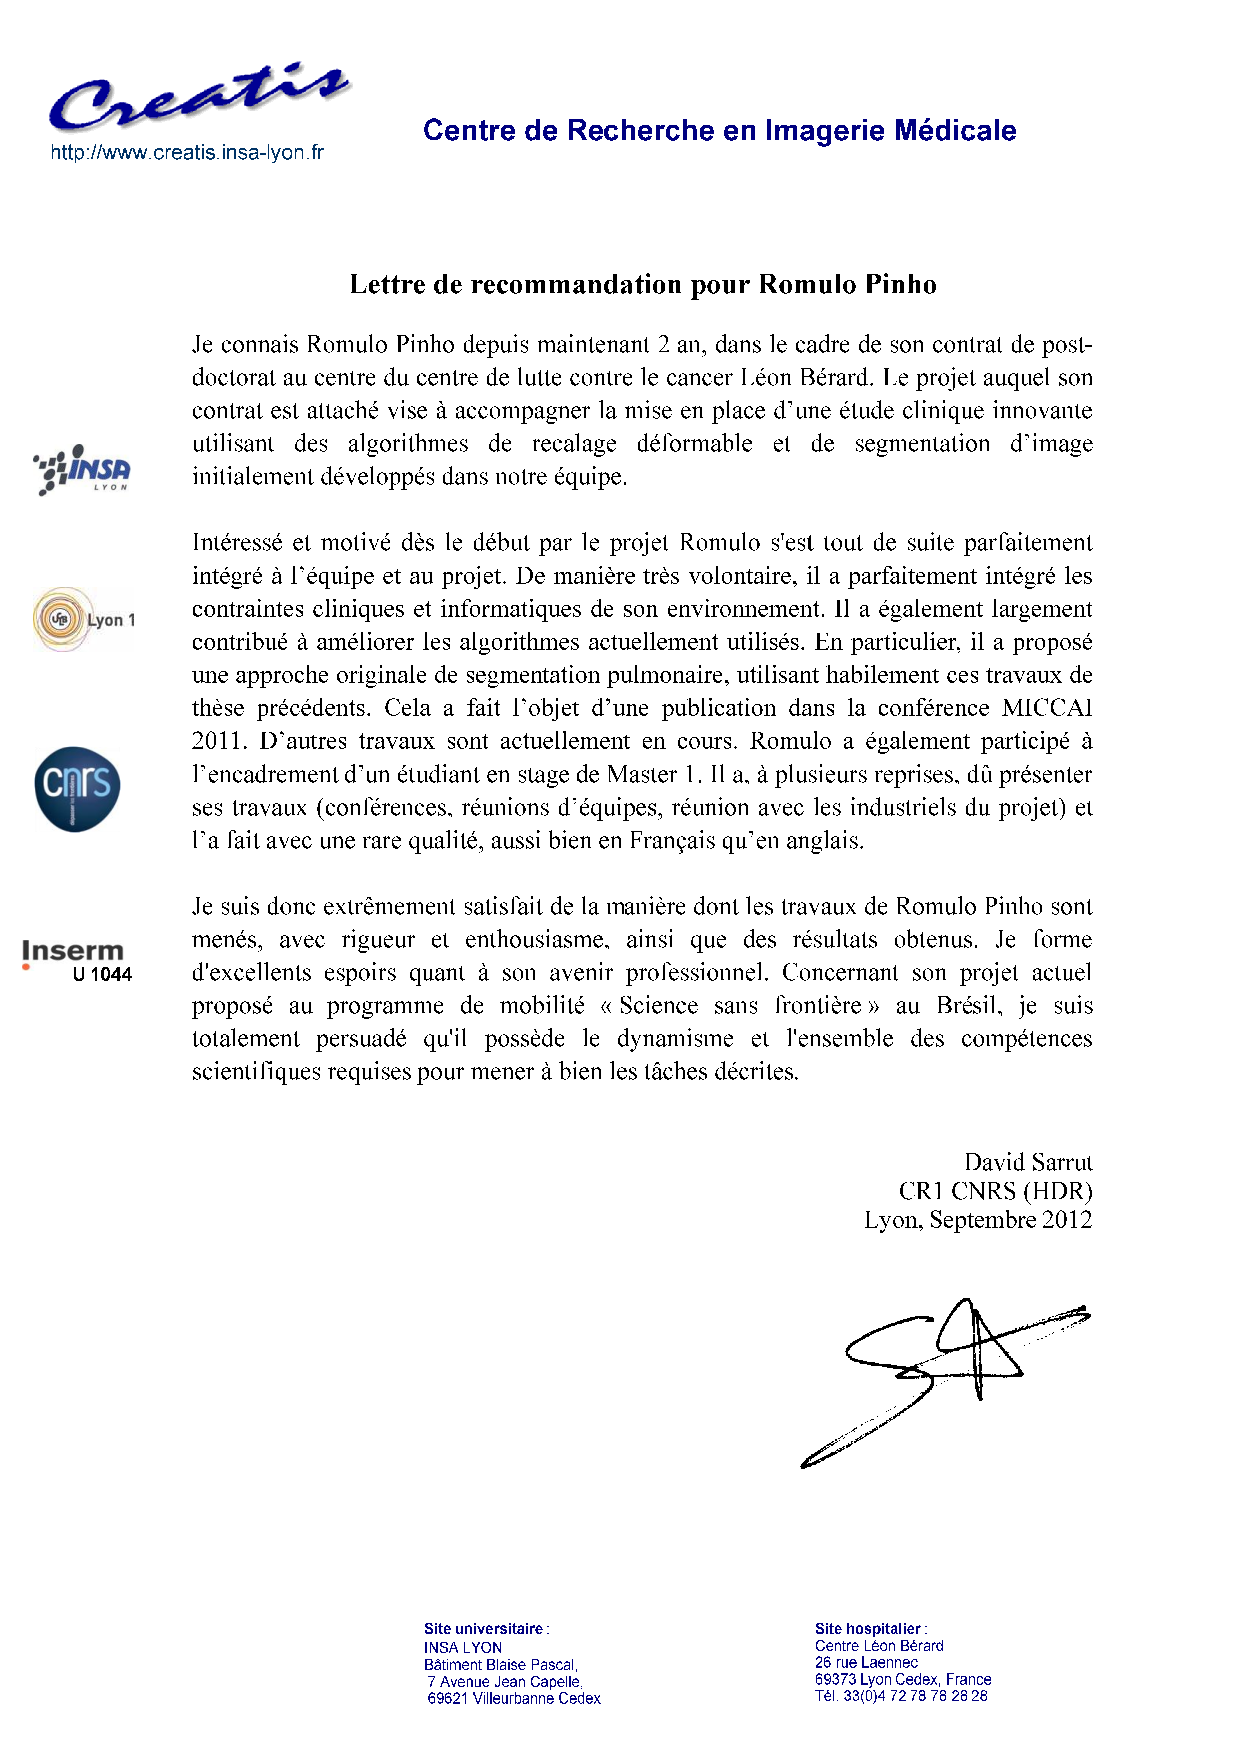
\includepdf[pages={1}]{david.pdf}
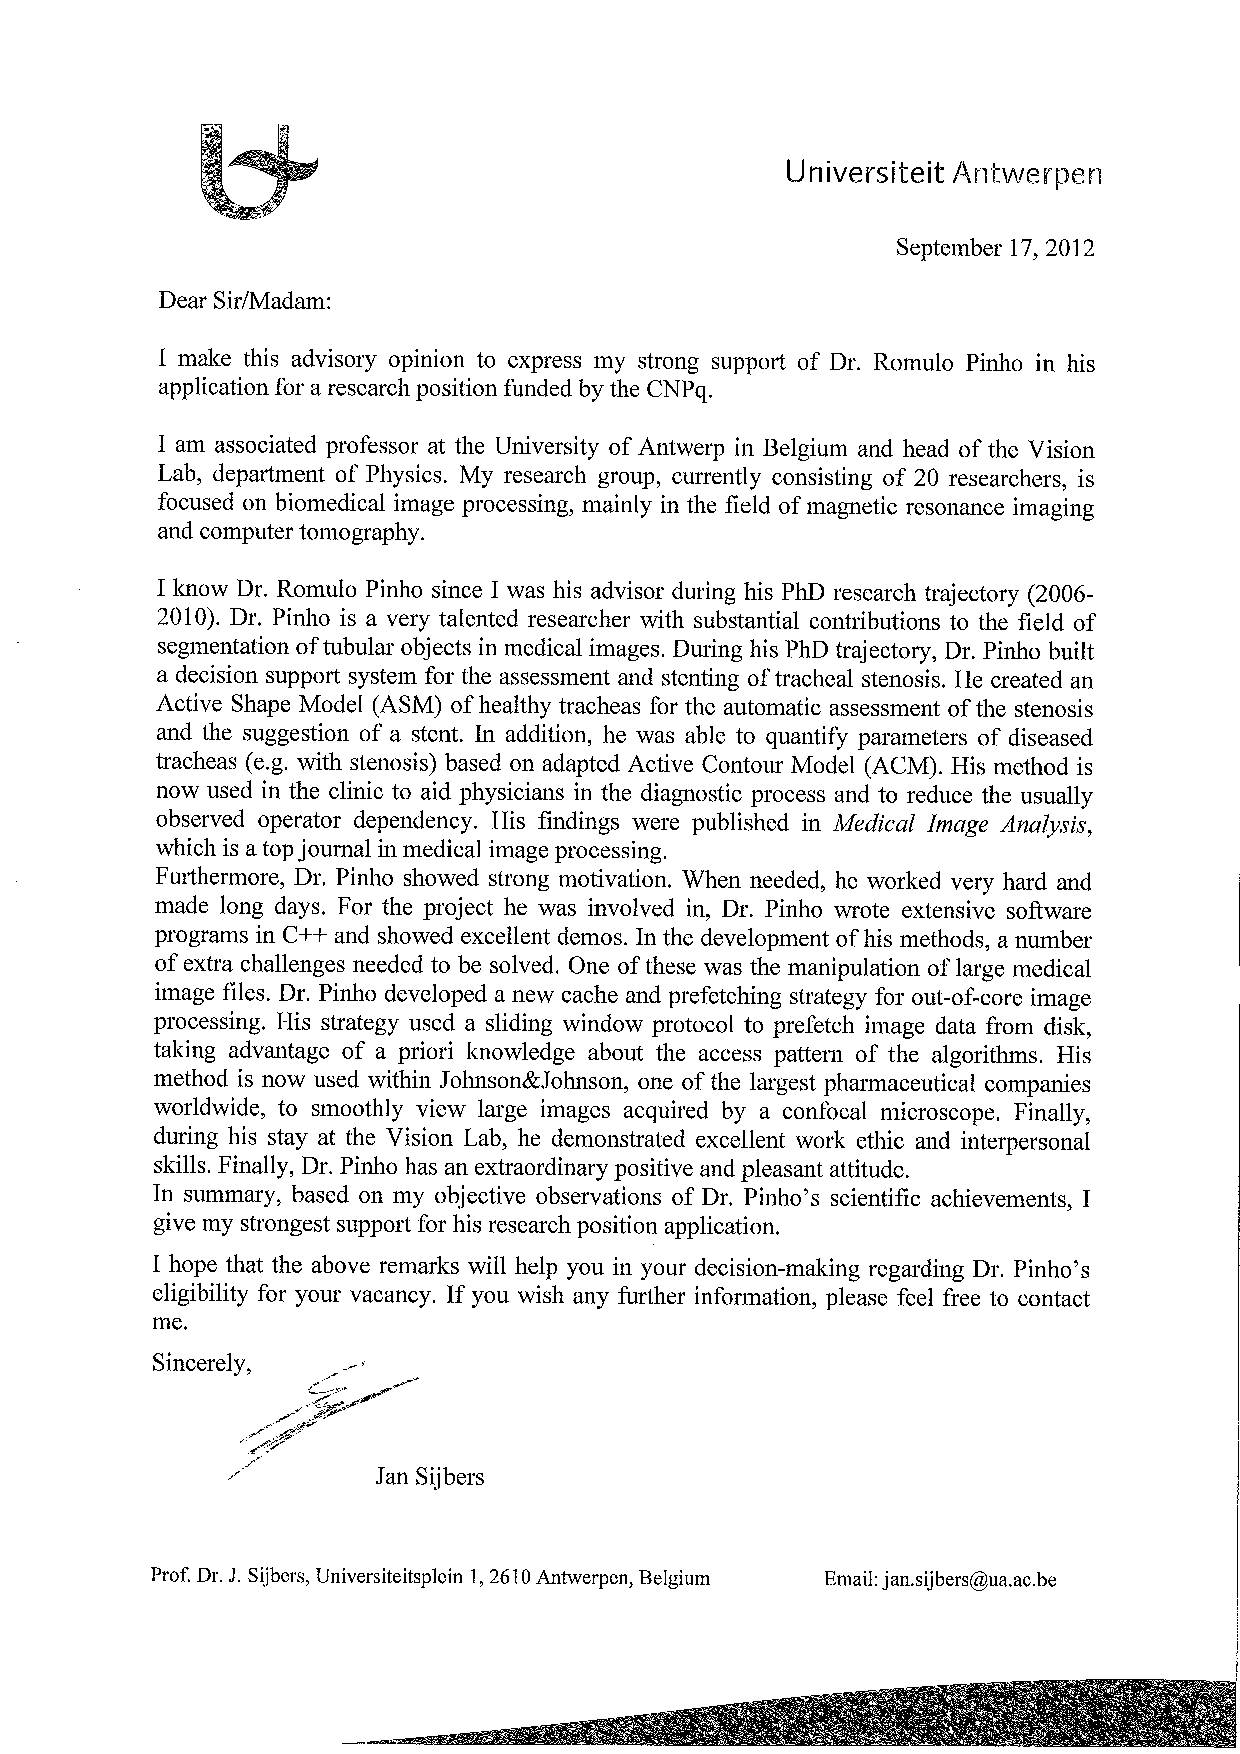
\includepdf[pages={1}]{jan.pdf}
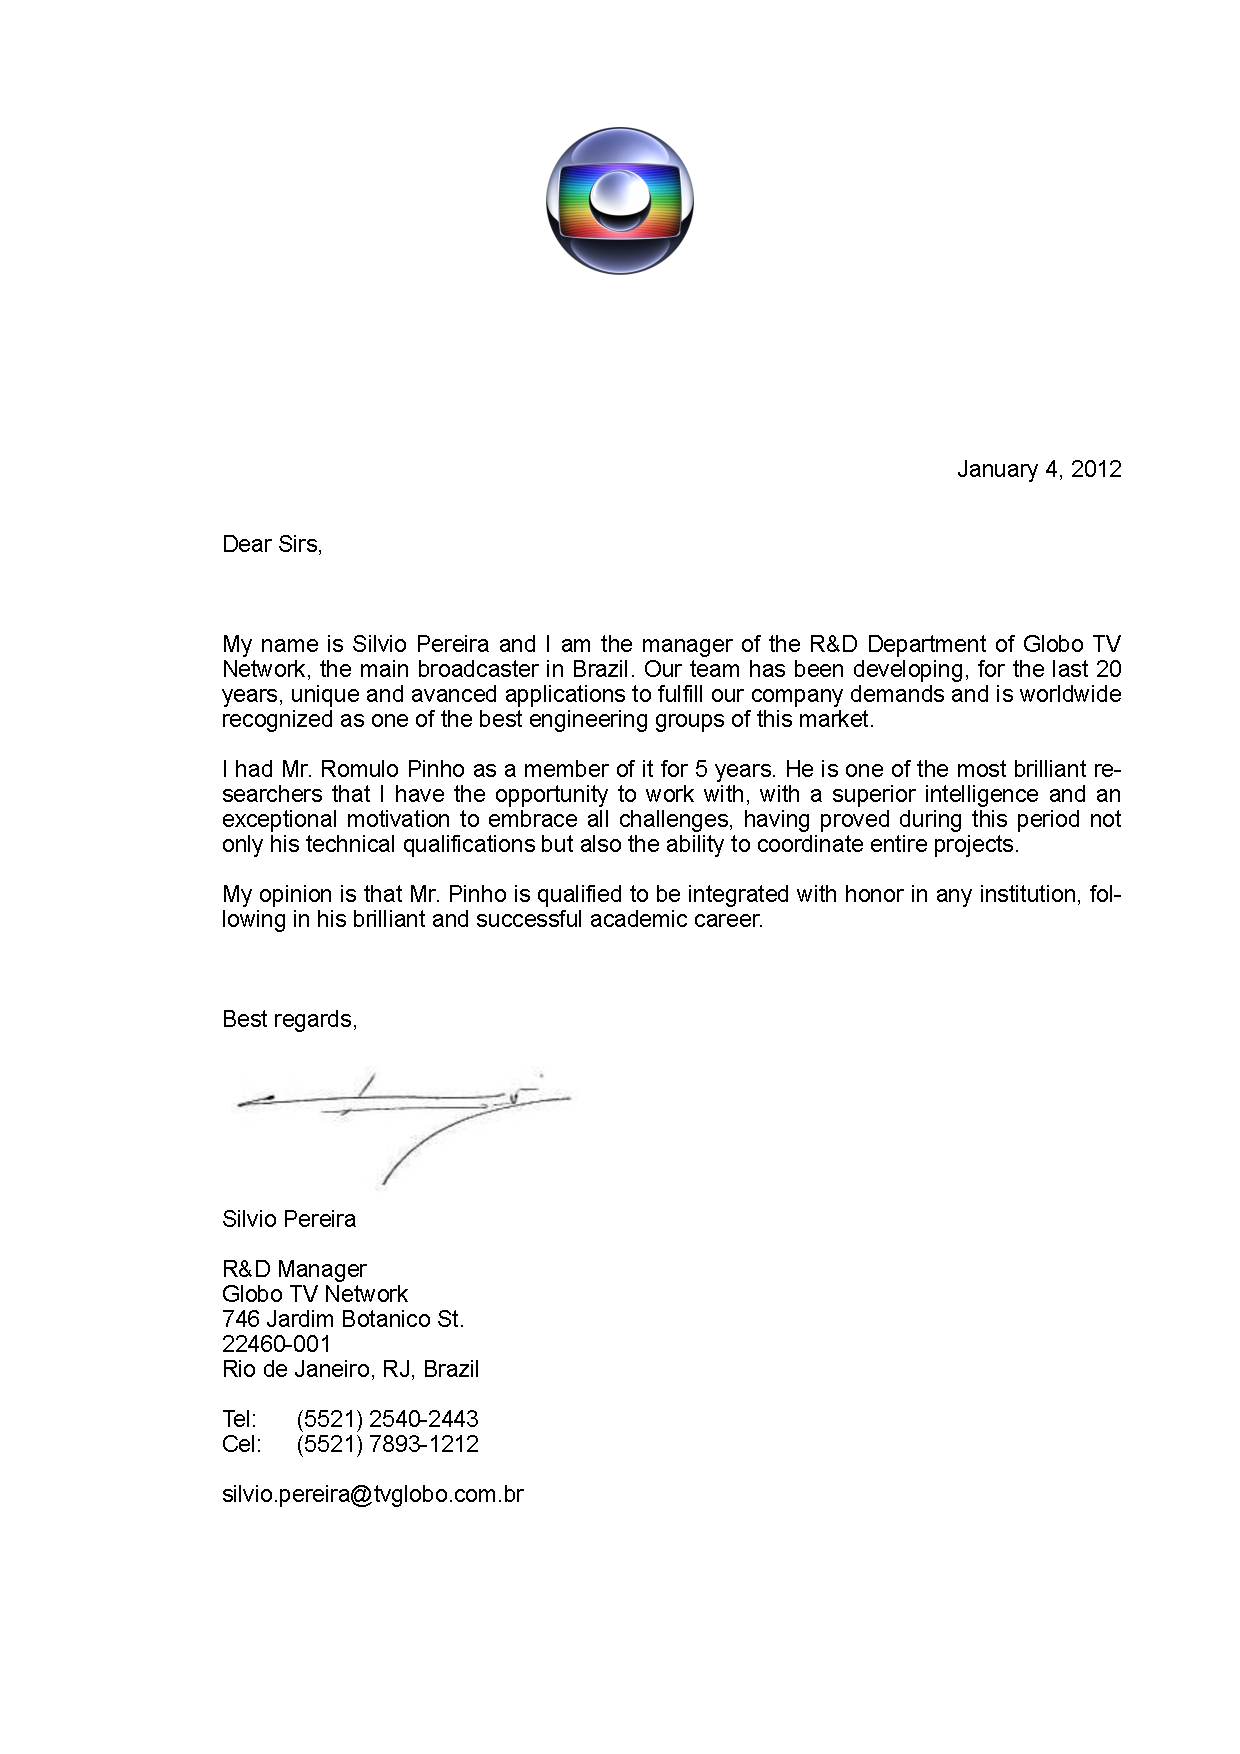
\includepdf[pages={1}]{silvio.pdf}
\includepdf[pages={1}]{joao.pdf}

%\section{Conclusions}


\end{document}
